\documentclass[conference]{IEEEtran}

\newcommand{\thetitle}{Towards Realistic Models of Wireless Workload}

\usepackage[pdftex]{graphicx}
\usepackage[labelfont=bf,small]{caption}
\usepackage[font=small,labelfont=bf,position=top,nearskip=0em]{subfig}
\usepackage{cite,amsmath,amssymb,rotating,multirow,bigstrut,url,wrapfig}
\usepackage[hyperfigures,bookmarks,bookmarksopen,bookmarksnumbered,frenchlinks=true,pdftitle={\thetitle}]{hyperref}

\hyphenation{op-tical net-works semi-conduc-tor IEEEtran}
\bibliographystyle{IEEEtran}

\newcommand{\email}[1]{$\left<{\textit{#1}}\right>$}
\newcommand{\caps}[1]{{\small{#1}}}

\title{
\vspace{-0.25em}
\thetitle
}
\author{
{\large{Stefan~Karpinski, Elizabeth~M.~Belding, Kevin~C.~Almeroth}} \vspace{0.25em}\\
Department of Computer Science \\
University of California, Santa Barbara \vspace{0.35em}\\
\textit{\{sgk,ebelding,almeroth\}@cs.ucsb.edu}
%\vspace{-0.5em}
}

\newcommand{\X}{\mathsf{X}}
\newcommand{\M}{\mathsf{M}}
\newcommand{\E}[1]{\left<#1\right>}
\newcommand{\abs}[1]{\left|#1\right|}
\newcommand{\R}{\mathbb{R}}
\newcommand{\Q}{\mathcal{Q}}
\newcommand{\ceil}[1]{\left\lceil#1\right\rceil}
\newcommand{\floor}[1]{\left\lfloor#1\right\rfloor}

\newcommand{\Trace}{\text{Trace}}
\newcommand{\TTT}{\text{TTT}}
\newcommand{\TTU}{\text{TTU}}
\newcommand{\TUU}{\text{TUU}}
\newcommand{\TUT}{\text{TUT}}
\newcommand{\UTU}{\text{UTU}}
\newcommand{\UTT}{\text{UTT}}

\newcommand{\figurename}{Figure}
\newcommand{\tablename}{Table}

\renewcommand{\topfraction}{0.95}% max fraction of floats at top
\renewcommand{\bottomfraction}{0.95}% max fraction of floats at bottom
\setcounter{topnumber}{4}
\setcounter{bottomnumber}{4}
\setcounter{totalnumber}{4}% 2 may work better
\setcounter{dbltopnumber}{4}% for 2-column pages
\renewcommand{\dbltopfraction}{0.9}	% fit big float above 2-col. text
\renewcommand{\textfraction}{0.07}% allow minimal text w. figs
\widowpenalty=1000
\clubpenalty=1000

\graphicspath{{plots/}}

\begin{document}
\maketitle

\begin{abstract}
Performance predictions from wireless networking laboratory experiments rarely seem to match what is seen once technologies are deployed. We believe that one of the major factors hampering researchers' ability to make more reliable forecasts is the inability to generate realistic workloads. To redress this problem, we take a fundamentally new approach to measuring the realism of wireless traffic models. In this approach, the realism of a model is defined directly in terms of how accurately it reproduces the performance characteristics of actual network usage. This cuts through the Gordian knot of deciding which statistical features of traffic traces are significant. We demonstrate that common experimental traffic models, such as uniform constant bit-rate traffic ({\footnotesize{CBR}}), drastically misrepresent performance metrics at all levels of the protocol stack. We also define and explore the space of synthetic traffic models, thereby advancing the understanding of how different modeling techniques affect the accuracy of performance predictions. Our research takes initial steps that will ultimately lead to comprehensive, multi-level models of realistic wireless workloads.
\end{abstract}

\section{Introduction}\label{sec:intro}

The evaluation of wireless technology requires the generation of workloads to test the viability and performance of the new protocol or technique being studied. We believe that lack of realism in traffic workload generation is one of the major limiting factors that prevents simulations and experimental network deployments from accurately predicting the real-world performance of wireless technologies. Today, very little is understood about the impact of different workloads on network performance. Uniform constant bit-rate traffic (\caps{CBR}) is commonly used to evaluate protocols, but there is no evidence that behavior under such workloads is an accurate predictor of performance under real usage patterns. The inability to experimentally forecast real-world performance is a severe handicap to the wireless networking community. It hinders the ability to effectively develop better solutions to the many difficult problems that face emerging wireless technologies.

This paper presents a fundamentally new approach to creating realistic models of workload in networks. Rather than subjectively choosing statistical measures that may or may not actually influence network performance, we define the realism of models directly in terms of their ability to accurately reproduce important metrics. We define a traffic model to be \textit{sufficiently realistic} with respect to a given performance metric, if the model produces metric values that are similar to those observed using the original trace to generate traffic.

The ultimate goal of this research is to take an observed trace of wireless traffic and reduce it to its essential characteristics, allowing researchers to generate arbitrary amounts of ``similar'' network traffic that exhibits the same performance properties as the original trace. This resulting synthetic model would also allow parameters to be altered for experimental purposes; changing, for example, the number of active nodes, the total number of flows, or the average data rate. This paper takes important first steps in understanding which aspects of the application-level traffic are essential, in the sense that they determine network performance, and which features are incidental, and may be altered without ill effect. % TODO: "More importantly, we provide a framework and methodology that paves the way for..."

Much research has studied usage patterns in both wired and wireless networks. A common feature of attempts to model traffic patterns has been that the choice of statistical characteristics to focus on is ultimately a matter of informed intuition. Unfortunately, the interaction of users and applications with the network seems to violate intuition more often than not, and simple models of behavior almost invariably fail~\cite{Paxson95,Royer01,Yoon03:speed-decay}. Recently, in the context of mobility, it has been shown that usage models can have a drastic impact on important performance metrics~\cite{Camp02,Yoon03:speed-decay,Yoon03:sound-models,Jardosh03,Zheng04}. In this work we explore the effect of traffic models, rather than mobility, upon network performance.
There is a large and diverse body of work on traffic analysis, modeling, and generation~\cite{Paxson95,Paxson96,Sommers04,Avallone04,Avallone06,Hernandez06}. Almost all of the traffic generation work has focused on wide-area Internet backbone traffic. The two most prominent traffic generation frameworks are Harpoon and \caps{D-ITG}. Harpoon~\cite{Sommers04} uses a traffic trace for self-training, and can subsequently generate synthetic traffic with certain statistical properties based on the original trace. \caps{D-ITG}~\cite{Avallone04,Avallone06} generates flows using a simple predefined (but configurable) independent sampling model for packet sizes and inter-packet intervals. While both Harpoon and \caps{D-ITG} provide excellent Internet traffic generation platforms, our results indicate that the properties modeled in these systems are not adequate for reproducing realistic performance in the wireless setting.

\section{Methodology}\label{sec:methodology}

Our general approach to understanding the realism of traffic models can be described as differential analysis with respect to performance metrics. The traces themselves serve as the control ``model'' of behavior, being the only known example of realistic workload. We study the impact of deviating from the trace behavior in various ways. Simulations are run using both the original trace traffic and corresponding traffic generated by synthetic models. For the comparison, we preserve as many features from the traces as each synthetic model will allow. For example, if a model alters the sizes of packets and inter-packet intervals, we ensure that the average packet size and average interval remain the same, so that the experimental comparison is fair. If the performance metrics of the synthetic model are significantly different from those of the original trace, then the model fails to capture the essential characteristics of traffic behavior. If the performance metrics are similar, we can conclude that the synthetic model abstracts away only non-essential traffic characteristics.

%In order to motivate the rest of our investigation, we must reveal some of our results early: the common synthetic models, such as variants on \caps{CBR}, drastically distort performance metrics at all levels of the protocol stack. Therefore, these simple models represent a lower bound on the realism that must be preserved by workload models in order to accurately predict performance. We must do better than these models if we want to have faith that our simulations actually predict anything meaningful. The essential question, then, is how to model real usage more accurately. Exploring the answer to that question is the concern of the rest of this paper.

\subsection{Trace Data \& Simulations}\label{sec:trace-data}\label{sec:simulations}

For our analysis, we use a 24-hour trace recorded in an infrastructured 802.11g wireless network with 18 access points deployed at the 60th Internet Engineering Task Force meeting (\caps{IETF}60), held in San Diego during August of 2004.  The traffic trace was captured using \texttt{\small{tcpdump}} at a single router, through which all wireless traffic for the meeting was routed, including traffic between wireless nodes. The snap length of the capture was 100 bytes, allowing all \caps{IP}, \caps{UDP} and \caps{TCP} headers to be analyzed. We limit our analysis to the 24-hour sub-trace recorded on Wednesday, August 4th. This trace contains a broad variety of behaviors and entails a very large volume of traffic: 2.1 million flows, 58 million packets, and 52 billion bytes.
% 2,085,563 flows, 58,377,994 packets of application data, and 51,988,245,537 bytes of application data.
Figure~\ref{fig:nodes-flows} shows the wide variations in the number of active flows and nodes over the course of the trace. This heterogeneity of behavior gives us greater confidence that success or failure of traffic models is not tied to any specific network condition or behavior, but is broadly applicable.

\begin{figure}[t]
\begin{center}
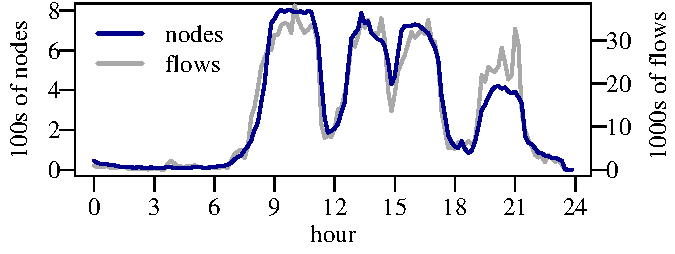
\includegraphics[width=3.5in]{nodes-flows}%
\vspace{-0.75em}%
\caption{The number of active nodes and flows over time.} 
\label{fig:nodes-flows}
\end{center}
\vspace{-2.25em}
\end{figure}

The first task is to extract application-level behavior from the trace header data. First, we split the trace into individual data flows. A flow is a series of packets sharing the following attributes: \caps{IP} and transport protocols (raw \caps{IP}, \caps{ICMP}, \caps{TCP}, \caps{UDP}); source and destination \caps{IP} addresses and \caps{TCP}/\caps{UDP} port numbers. Next, the quantity of application-initiated data contained in each packet is calculated. For non-\caps{TCP} packets, this quantity is simply the size of the transport-layer payload, but for \caps{TCP} the calculation is more complicated: only new data transfers, explicitly initiated by the application, are counted. Data retransmitted by TCP is disregarded, and empty ACKs are ignored. SYN and FIN flags in packets (even empty ones) are counted as a byte each, since they are explicitly signaled by the application.
After processing, we have a collection of flows, each with a sequence of timestamps and the amount of application-initiated data sent at that time.

We use the Qualnet wireless network simulator to perform our experiments. We simulate a stationary multi-hop 802.11g network using the Ad hoc On-demand Distance Vector (\caps{AODV}) routing protocol~\cite{rfc:aodv}, with nodes placed randomly in a square field with sides of 150 meters. In addition to the active nodes corresponding to trace \caps{IP}s, half as many ``infrastructure'' nodes are added to each simulation: these nodes initiate no data, and simply serve as additional network relays. Our simulations resemble 802.11 multi-hop mesh networks of the kind that are increasingly studied and deployed for the delivery of broadband access in residential, corporate or conference settings.

One possible point of objection to our methodology is that we use infrastructured trace data to drive multi-hop network simulations. Other potential objections stem from disregarding the interaction of different aspects of the original network: \caps{TCP} feedback, physical environment, node mobility, and handover behavior. While it is true that these aspects all influence traffic patterns and performance, being able to approximate traffic behavior accurately in isolation is still far better than not being able to approximate it at all, which is the current situation. Before we can hope to understand the interaction between workload and other aspects of network behavior, we must study traffic patterns alone and learn to model them without additional complicating factors. Finally, we study a multi-hop wireless network because it is more sensitive to workload, and thus serves as a more delicate tool to measure the impact of traffic models.

%There is a natural inclination among networking researchers to try to reproduce all aspects of the original wireless setting in which a trace was recorded. We typically want to reproduce all aspects of the original setting as accurately as we can: application-level traffic, the full protocol stack, \caps{TCP} feedback behavior, the physical environment, node mobility, handover behavior, etc. The intuition behind this inclination is that all these aspects interact in a complex manner to produce the somewhat mysterious gestalt behavior that is ultimately observed in the network. In our minds these many levels are all inextricably linked.

%In this research, however, we are not trying to reproduce the wireless behavior of the original network in which our traces were recorded---we have already observed that directly. Instead, we isolate the application-level behavior observed, and use it to explore the nature of realism in this one aspect of network behavior. The goal is to understand aspects of the application-level traffic are characteristic in the sense that they determine the network performance, while other features are incidental, and may be altered without any effect.

The 24-hour trace is split into 144 10-minute segments, each of which serves as the basis for a set of simulations using different traffic models. We present the various traffic models in Section~\ref{sec:models-metrics}. To preserve the fairness of the performance comparison, we keep as many features as possible constant across different traffic models. The traffic generated by each synthetic model preserves as many characteristics from the original trace as possible, within the constraints of the model. Moreover, for each 10-minute segment, the following features are preserved across all models: the numbers of wireless nodes, the number of flows, the number of application-initiated data units sent, the total bytes of application data sent, and the average flow duration (and therefore the average data rate).

\subsection{Traffic Models \& Performance Metrics}\label{sec:models-metrics}

\begin{figure*}[tb]
\begin{center}
\subfloat[trace topology]
{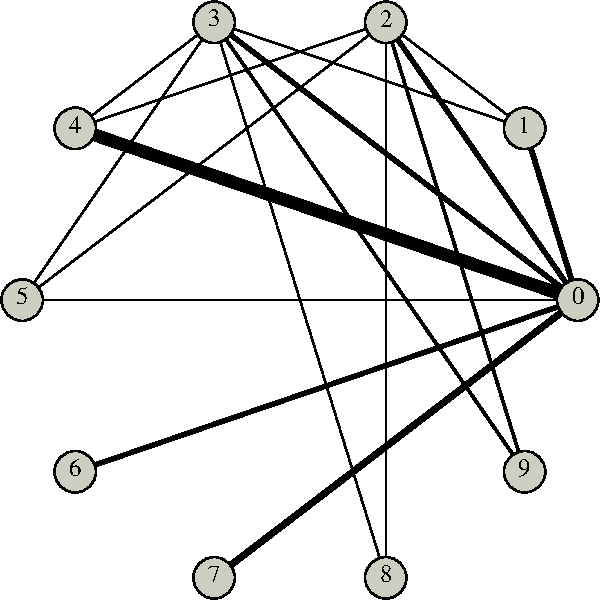
\includegraphics[width=1.392in]{flow_topology_trace}\label{fig:flow-topology-trace}}
\subfloat[random topology]
{\includegraphics[width=1.392in]{flow_topology_uniform}\label{fig:flow-topology-uniform}}
\subfloat[trace flows]
{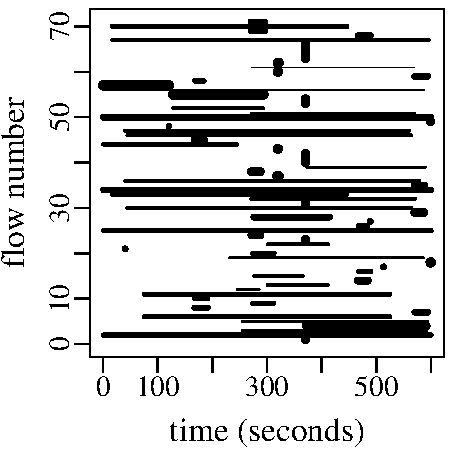
\includegraphics[width=1.392in]{flow_behavior_trace}\label{fig:flow-behavior-trace}}
\subfloat[uniform flows]
{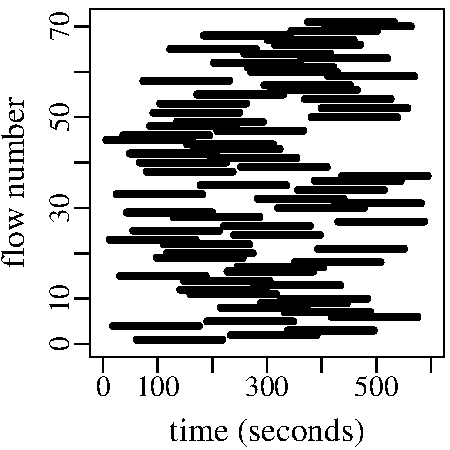
\includegraphics[width=1.392in]{flow_behavior_uniform}\label{fig:flow-behavior-uniform}}
\subfloat[packet behavior]
{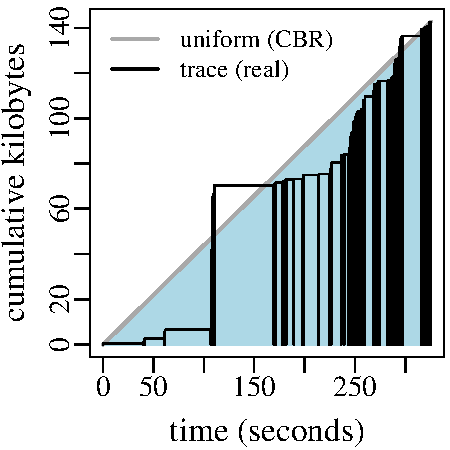
\includegraphics[width=1.392in]{flow_packet_behavior}\label{fig:packet-behavior}}
\caption{Examples illustrating the different traffic models for the three levels of behavior. Figures \ref{fig:flow-topology-trace} and \ref{fig:flow-topology-uniform} show example flow topologies. The width of each line is proportional to the logarithm of the number of flows between the nodes it connects (zero is the Internet gateway). Uniform and trace flow behavior examples are plotted in Figures \ref{fig:flow-behavior-trace} and \ref{fig:flow-behavior-uniform}. The time axis indicates when flows start and end; the width of each flow line is proportional to the logarithm of its data rate. Figure \ref{fig:packet-behavior} compares \caps{CBR} packet behavior with the trace of an actual flow. In the uniform model, the cumulative data sent increases smoothly over time, whereas in the actual packet trace, the transmissions are variable both in size and in inter-packet interval, leading to a ``lumpy'' cumulative data plot.}
\label{fig:traffic-models}
\end{center}
\vspace{-2em}
\end{figure*}

Traffic generation models determine three orthogonal levels of traffic behavior:
\begin{enumerate}
\item \textbf{Flow End-Point Topology}: which nodes communicate with each other, and how frequently; i.e. how flow end-points are mapped onto nodes in the network.
\item \textbf{Flow Behavior}: high-level parameters for each flow; including start time, end time, packets sent, bytes sent.
\item \textbf{Packet Behavior}: sizes of individual packets, and the interval between their transmission.
\end{enumerate}
Examples of different behaviors at each level are illustrated in Figure~\ref{fig:traffic-models}. For instance, Figures~\ref{fig:flow-topology-trace} and \ref{fig:flow-topology-uniform} show the difference between the layout of flow communication in an actual trace scenario as compared with the layout when the same flows are distributed randomly between end-points.

We consider the following two traffic models because they are the ones most commonly used to generate workload in wireless experiments:
\begin{itemize}
\item \textbf{RandomUniform\caps{CBR}}: flows are \caps{CBR}, and all have equal duration, packet count, and bit-rate. The end-points and start times are chosen randomly.
\item \textbf{Uniform\caps{CBR}}: the same as RandomUniform\caps{CBR}, but the end-points of each flow are taken from the trace.
\end{itemize}
These two models serve as reference points for our exploration of the traffic models. Their inclusion also allows us reason about the accuracy of current evaluations.

We explore the space of synthetic models starting from both the top (end-point topology) and the bottom (packet behavior). The following models alter only packet behavior:
\begin{itemize}
\item \textbf{\caps{CBR}}: constant bit-rate; within each flow, packets are all the same size and all inter-packet intervals are equal.
\item \textbf{SampleTime}: a per-flow histogram of inter-packet intervals is used to randomly generate synthetic packet behavior; packet sizes from the trace are used.
\item \textbf{SampleSize}: the same as SampleTime, but sampling packet sizes instead of inter-packet intervals.
\item \textbf{SampleTimeSize}: both inter-packet intervals and packet sizes are sampled from histograms independently.
\end{itemize}
Note that variable bit-rate (\caps{VBR}) traffic models, sometimes used for audio, video or voice traffic, are simply special cases of one of the last three models.\footnote{\scriptsize{VBR} models are typically used with a single fixed distribution of intervals and sizes for all flows. Greater fidelity is expected here since each flow is modeled with the exact distribution of its trace behavior. In further research, we have found that using {\scriptsize{VBR}} with a single distribution across all flows distorts performance nearly as much {\scriptsize{CBR}} does.}

We also consider the following traffic models that alter only the flow end-point topology:
\begin{itemize}
\item \textbf{ShuffleEndPoints}: permutes the flow end-points; this is equivalent to permuting the locations of nodes.
\item \textbf{RandomEndPoint}: choose random end-points for each flow, each node having equal probability.
\item \textbf{SampleEndPoint}: flow end-points are sampled from independent histograms of source and destination nodes.
\item \textbf{SampleEndPointsJoint}: flow end-points are sampled from a joint histogram of source-destination pairs.
\end{itemize}

In order to evaluate the realism of these traffic models, we have selected four commonly used performance metrics at different layers of the protocol stack:
\begin{enumerate}
\setlength{\itemsep}{0em}
\item \textbf{Application:} end-to-end delay and received throughput.
\item \textbf{Network:} \caps{AODV} control overhead (\caps{RREQ/RREP/RERR}).
\item \textbf{Link (\caps{MAC}):} packet retransmission rate.
\end{enumerate}

\section{Results}\label{sec:results}

\begin{figure*}[htb]
\subfloat[\textbf{Application:} Average End-to-End Delay]%
{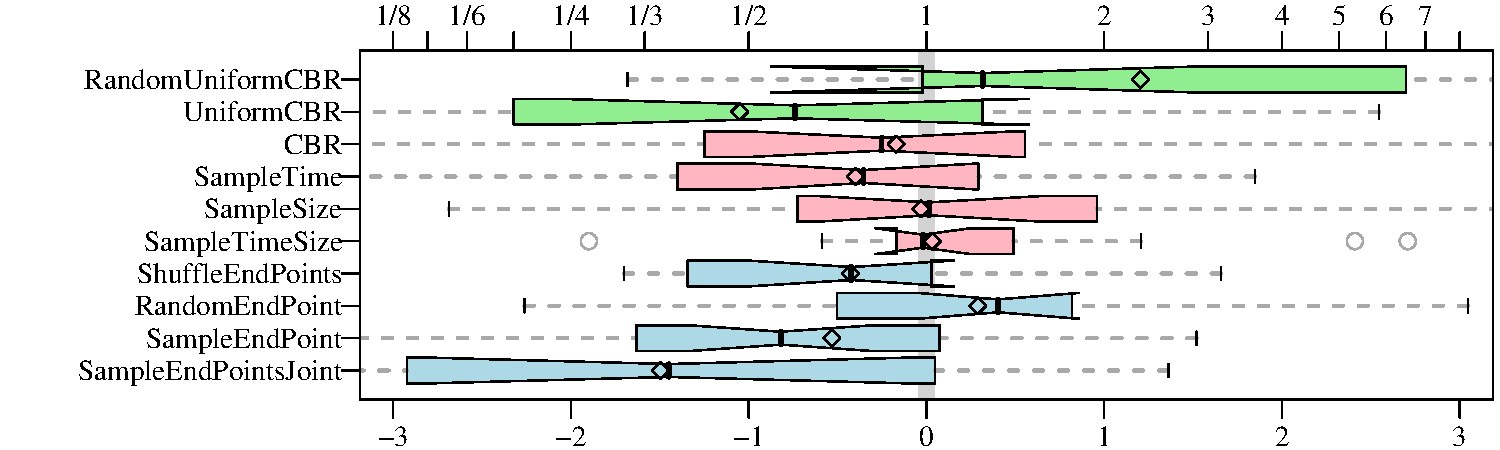
\includegraphics[width=3.55in]{plots/Application/Average_Delay.pdf}}%
\subfloat[\textbf{Application:} Total Received Throughput]%
{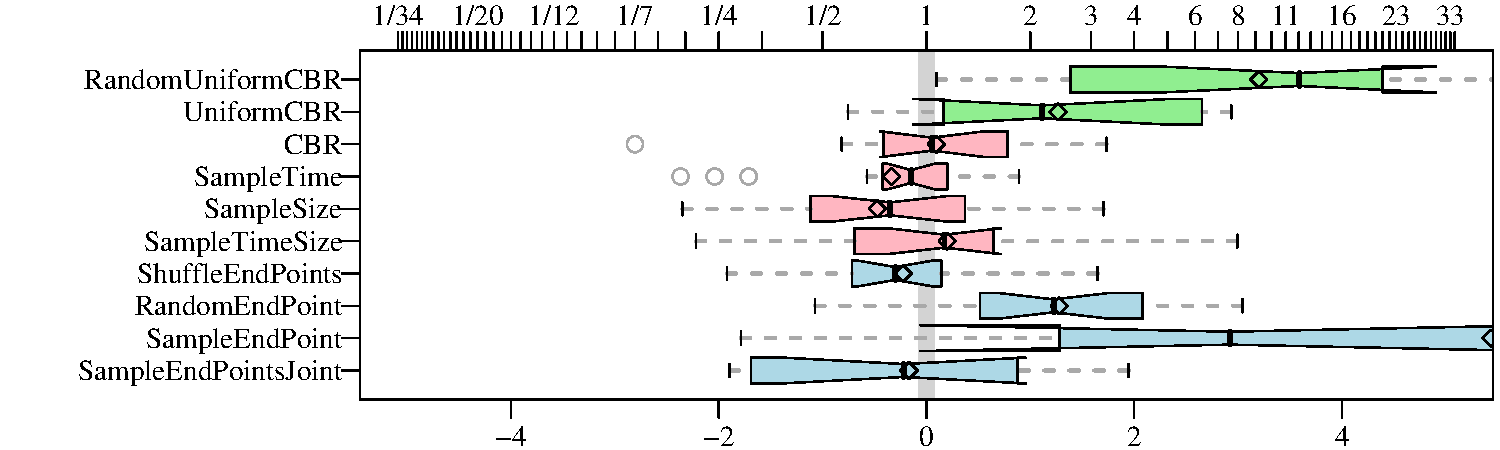
\includegraphics[width=3.55in]{plots/Application/Received_Throughput.pdf}}
\subfloat[\textbf{Network:} AODV Control Overhead]%
{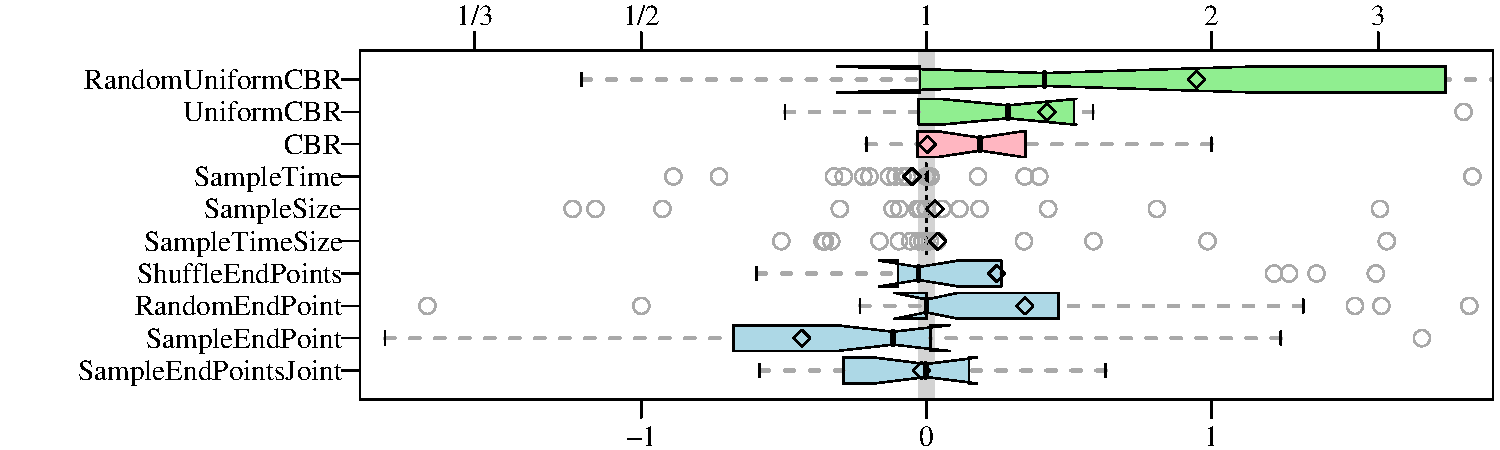
\includegraphics[width=3.55in]{plots/Network/Control_Overhead.pdf}}%
\subfloat[\textbf{Link (MAC):} Retransmission Rate]%
{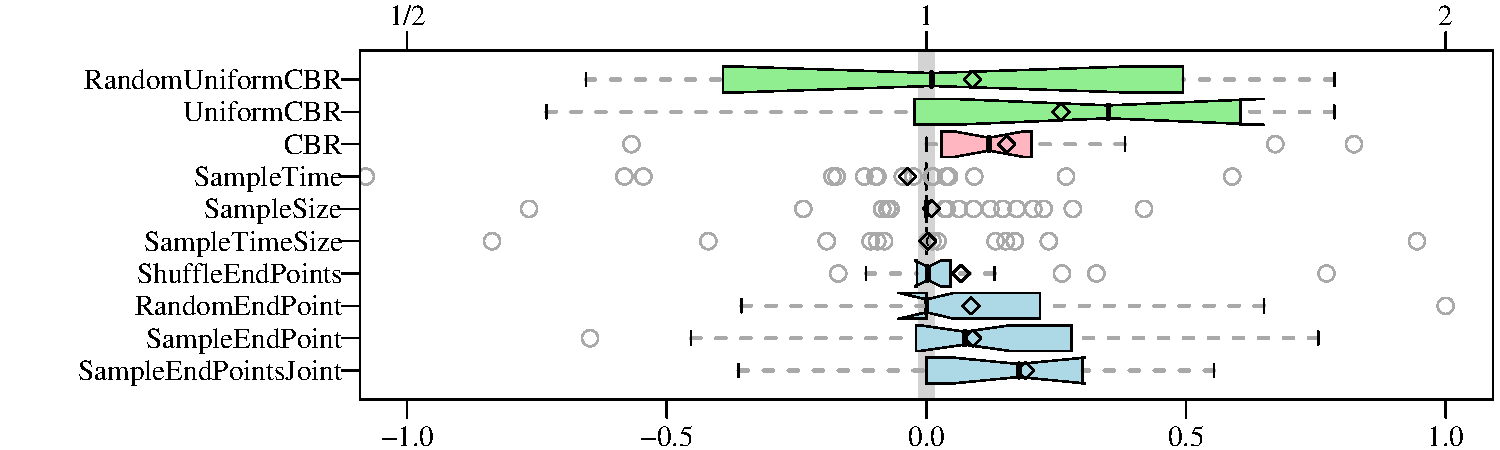
\includegraphics[width=3.55in]{plots/MAC/Retransmissions.pdf}}%
\caption{Box-and-whisker plots of log-ratio error values for all metrics and traffic models. The lower axis indicates the log-ratio, while the upper axis shows raw ratio values. Each box contains the central majority of log-ratio values: the left and right bounds are at the $25^\text{th}$ and $75^\text{th}$ percentiles. The dark middle line indicates the median value, while the diamond marks the mean. The whiskers (dotted lines) extend to the furthest non-outlier values, while the points beyond that are outliers. The notch in the middle of each bar indicates a $95\%$ confidence interval for the true underlying median value; if two notches do not overlap, they are very unlikely to have the same median.}
\label{fig:box-plots}
\vspace{-1.25em}
\end{figure*}

Our experimental results are summarized in Figure~\ref{fig:box-plots}. Box-and-whisker plots are a common way of concisely summarizing distributions of values. The values summarized in this case are the error ratios of the four metrics in each of the 144 simulation scenarios simulated. The error ratio for a scenario is the metric value observed using the alternate traffic model divided by the value observed using trace traffic. The error ratios are plotted on a log-scale (shown under each set of plots); this makes underestimation by some factor symmetric with overestimation by the same factor. A traffic model that realistically represents a performance metric should have a narrow box, centered around the middle line, indicating error ratios generally close to unity. If the box is too wide, the values are highly unreliable; if the box is not centered, the metric in question is being consistently misrepresented.

To begin our analysis, we examine the most common model used to generate experimental workloads: RandomUniform\caps{CBR}. In this model, all aspects of flow behavior are homogeneous---all flows have the same number of packets, duration, and data rate. Each flow is a steady stream of identical packets. The end-points of streams are randomly selected, and the start time of each stream is chosen randomly. This traffic model drastically skews every single performance metric we present, as well as others not shown. More than half of the time, received throughput is overestimated by more than seven times; 70\% of the time, it is overestimated by more than a factor of two. This case demonstrates the need for this research: \textit{this common traffic model is not effectual for predicting general network performance under real usage conditions}. The Uniform\caps{CBR} model provides a significant improvement in representation accuracy, but still skews all metrics considerably. The improvement, however, demonstrates that simply understanding which nodes talk to each other and with what frequency can significantly improve the accuracy of performance predictions.

Next, we consider models that only deviate from the trace by altering packet behavior: \caps{CBR}, SampleTime, SampleSize, and SampleTimeSize. These models should be fairly accurate, since they are using real flow behavior (duration, packet count, data rate), and end-point topology, synthesizing only the sizes and intervals of individual packets within each flow. Despite the limited domain of synthesis, \caps{CBR} traffic does not fare well: it underestimates average delay by 30\% more than half of the time, and by 40\% on average. \caps{CBR} appears to fare better for network and link-layer metrics, until one notes that the other models all achieve near-perfect accuracy for these metrics. The star traffic model of this category is the SampleTimeSize model: it has mean and median error values near unity for every metric, and consistently has a small box width. Interestingly, sampling only time or size does not yield better results---it is better to sample both, independently. The conclusions to be drawn from these models are: 1) \caps{CBR}, even with completely realistic higher level behavior, is a poor model for generic wireless network traffic; 2) neither packet sizes, nor inter-packet intervals need to be modeled with time-series---it is adequate to simply sample each repeatedly, from a single distribution, so long as that distribution is realistic.

The metrics that alter only end-point topology are ShuffleEndPoints, RandomEndPoint, SampleEndPoint, and SampleEndPointsJoint. The ShuffleEndPoints model serves as a control for this group of models because the flow topology generated is isomorphic to that of the original trace, with only the physical locations of nodes permuted. It should---and does---have median error values close to unity. Moreover, the size and shape of the error distribution for this model dictates how well other models should represent metrics: if a synthetic model accurately captures the essential topological characteristics, it should have an error distribution similar to the ShuffleEndPoints model. None of the other models fares particularly well here: they each fail at one level or another. Unlike the case of packet behavior, we cannot simply sample the empirical topology pattern and achieve realistic behavior. More advanced topology models must be developed to capture the intricate patterns of connecting nodes in real networks.

\section{Conclusions}\label{sec:conclusions}

This paper represents the first steps toward understanding the complexities of how traffic workload affects performance metrics in wireless networks. There are three immediate, concrete conclusions we can draw:
\begin{enumerate}
\item Packet behavior does not require complex, time-series models to accurately reproduce performance under real workloads. If the higher levels of traffic are properly modeled, a simple independent sampling approach will work for both packet sizes and inter-packet intervals.
\item Flow end-point topology, or which nodes talk to each other and how frequently, does require complex modeling, at least beyond the simple sampling approaches attempted here.
\item Common traffic models such as RandomUniform\caps{CBR} are inadequate for modeling real workload. Performance assessments made using such models are potentially off by as much as an order of magnitude.
\end{enumerate}
A far more important contribution of this work, however, is the general framework and methodology it provides for exploring the realism of traffic models. Our approach promises to yield rich results, culminating in comprehensive, multi-level traffic models that can reliably generate  wireless workload that accurately represents real-world usage. We are currently extending sampling-based packet models to the levels of flow behavior and end-point topology. This extension requires the development of new data-mining techniques that allow discovery of behavioral similarities across flows. These techniques promise to provide highly general techniques for distilling the essential characteristics of network traffic. With realistic, multi-level traffic models models, the networking community will be able to make confident performance predictions from experimental evaluations.

\section{Acknowledgments}
This work was funded in part by NSF Career Award CNS-0347886 and by NSF NeTS Award CNS-0435527.

\bibliography{IEEE,references}

\end{document}
